\chapter[Leçon 37: Conditionnel, Zäiten a Beweegungsausdréck]{Leçon 37: De Conditionnel (Présent \& Passé), Zäiten a Beweegungsausdréck}

Dës Lektioun baséiert op engem interaktive Cours a behandelt fundamental Strukture vun der Lëtzebuerger Grammaire an alldeegleche Kommunikatioun. Mir kucken eis d'Reegele fir d'Prepositioune mat der Beweegung un (\textit{goen an d'Stad}, \textit{op Esch}, \textit{op d'Maldiven}), d'Kombinatioun vu \textit{goen} mat engem zweeten Infinitiv (\textit{akafe goen}, \textit{schlofe goen}), an Ausdréck fir Zoustandsverännerunge mat \textit{ginn} (\textit{verréckt ginn}, \textit{kribbeleg ginn}, \textit{ënnergoen}). Dono maache mir eng grëndlech a separat Analys vum \textbf{Conditionnel présent} an dem \textbf{Conditionnel passé} mat Referenz op d'INL-Léierbicher (\textit{Schwätzt dir Lëtzebuergesch? B1}), léieren de wichtegen Ënnerscheed tëscht \textit{fueren}, \textit{féieren} a \textit{feieren}, klären \textit{heem} an \textit{doheem}, an entdecken déi kulturell Bedeitung vum Wuert \textbf{d'Joffer}.

\textit{Cette leçon est consacrée à des structures grammaticales et lexicales incontournables du luxembourgeois parlé et écrit. Nous étudions les prépositions de mouvement (\textbf{goen an d'Stad}, \textbf{op Esch}, \textbf{op d'Inselen}), la combinaison de \textbf{goen} avec un second infinitif (\textbf{akafe goen}, \textbf{schlofe goen}), et les expressions d'état avec \textbf{ginn} (\textbf{verréckt ginn}, \textbf{kribbeleg ginn}, \textbf{ënnergoen}). Nous consacrons ensuite une étude détaillée et séparée au \textbf{conditionnel présent} et au \textbf{conditionnel passé} en nous appuyant sur les manuels de référence de l'INL (\textit{Schwätzt dir Lëtzebuergesch? B1}), avant de distinguer \textbf{fueren}, \textbf{féieren} et \textbf{feieren}, de différencier \textbf{heem} et \textbf{doheem}, et d'aborder la portée culturelle du terme \textbf{d'Joffer}.}

\textit{This lesson is dedicated to essential grammatical and conversational building blocks of Luxembourgish. We cover prepositions of direction and movement (\textbf{goen an d'Stad}, \textbf{op Esch}, \textbf{op d'Inselen}), pairing \textbf{goen} with a second infinitive (\textbf{akafe goen}, \textbf{schlofe goen}), and state-change expressions with \textbf{ginn} (\textbf{verréckt ginn}, \textbf{kribbeleg ginn}, \textbf{ënnergoen}). We then provide an in-depth, separate examination of both the \textbf{conditional present} and \textbf{conditional past} based on official INL reference textbooks (\textit{Schwätzt dir Lëtzebuergesch? B1}), followed by clarifying the distinction between \textbf{fueren}, \textbf{féieren}, and \textbf{feieren}, contrasting \textbf{heem} vs \textbf{doheem}, and exploring the cultural meaning of \textbf{d'Joffer}.}

\vspace{1.5em}

\section[Prepositioune mat goen / Prepositions of Direction]{Prepositioune mat der Beweegung (goen) \\/ Prépositions de mouvement et de direction \\/ Prepositions of Movement and Direction}

Wann een sech iergendwouhi beweegt (mat de Verbe \textit{goen}, \textit{fueren}, \textit{lafen}), ännert d'Prepositioun jee no der Destinatioun :

\textit{Lorsque l'on exprime un déplacement vers un lieu (avec les verbes \textit{goen}, \textit{fueren}, \textit{fléien}), la préposition employée varie selon qu'il s'agit de la capitale, d'une autre localité du pays, d'un pays ou d'une île :}

\textit{When expressing movement towards a destination (with verbs such as \textit{goen}, \textit{fueren}, \textit{fléien}), the preposition used depends on whether you are heading to the capital, another town in Luxembourg, a country, or an island:}

\begin{itemize}
    \item \textbf{D'Haaptstad (La capitale / The capital) $\rightarrow$ an (+ Akkusativ)} :
    \begin{itemize}
        \item \textit{Ech ginn \textbf{an d'Stad}.} $\rightarrow$ \textit{FR :} Je vais en ville (à Luxembourg-Ville). / \textit{EN :} I am going to the city (Luxembourg City).
        \item \textit{Opgepasst op d'Positioun (Attention à la position / Note on location -- Dativ) :} \\
        \textit{Ech sinn \textbf{an der Stad}.} $\rightarrow$ \textit{FR :} Je suis en ville. / \textit{EN :} I am in the city.
    \end{itemize}

    \vspace{0.4em}

    \item \textbf{Aner Uertschaften a Stied zu Lëtzebuerg $\rightarrow$ op} :
    \begin{itemize}
        \item Fir quasi all aner Uertschaft am Grand-Duché benotzt een d'Prepositioun \textbf{op} : \\
        \textit{FR :} Pour presque toutes les autres localités du pays, on emploie la préposition \textbf{op} : \\
        \textit{EN :} For almost all other towns and villages in the country, the preposition \textbf{op} is used:
        \item \textit{Ech ginn \textbf{op Esch}.} $\rightarrow$ \textit{FR :} Je vais à Esch-sur-Alzette. / \textit{EN :} I am going to Esch.
        \item \textit{Hie fiert \textbf{op Iechternach}.} $\rightarrow$ \textit{FR :} Il va à Echternach. / \textit{EN :} He drives to Echternach.
        \item \textit{Mir ginn \textbf{op Dikrech} / \textbf{op Waasserbëlleg} / \textbf{op Jonglënster}.} \\
        $\rightarrow$ \textit{FR :} Nous allons à Diekirch / à Wasserbillig / à Junglinster. \\
        $\rightarrow$ \textit{EN :} We are going to Diekirch / to Wasserbillig / to Junglinster.
        \item \textit{Humoristescht Beispill aus dem Cours :} \textit{Ech ginn \textbf{op de Mars}} / \textit{Ech ginn \textbf{op de Mound}} ! \\
        $\rightarrow$ \textit{FR :} Exemple humoristique du cours : Je vais sur Mars / Je vais sur la Lune ! \\
        $\rightarrow$ \textit{EN :} Humorous classroom example: I am going to Mars / I am going to the Moon!
    \end{itemize}

    \vspace{0.4em}

    \item \textbf{Länner (Pays / Countries) $\rightarrow$ an / a} :
    \begin{itemize}
        \item \textbf{Neutral Länner ouni Artikel (Pays neutres sans article / Neuter countries without article) :}
        \begin{itemize}
            \item \textit{Ech ginn \textbf{an Däitschland}.} $\rightarrow$ \textit{FR :} Je vais en Allemagne. / \textit{EN :} I am going to Germany.
            \item \textit{Ech ginn \textbf{a Frankräich}.} $\rightarrow$ \textit{FR :} Je vais en France. / \textit{EN :} I am going to France.
            \item \textit{Ech ginn \textbf{an England}.} $\rightarrow$ \textit{FR :} Je vais en Angleterre. / \textit{EN :} I am going to England.
        \end{itemize}
        \item \textbf{Weiblech Länner mat Artikel (Pays féminins avec article / Feminine countries with article) :}
        \begin{itemize}
            \item \textbf{d'Belsch} (f.) : \textit{Ech ginn \textbf{an d'Belsch}} (Direktioun / direction : \textit{FR :} Je vais en Belgique. / \textit{EN :} I am going to Belgium.) vs \textit{Ech sinn \textbf{an der Belsch}} (Positioun / position : \textit{FR :} Je suis en Belgique. / \textit{EN :} I am in Belgium.).
            \item \textbf{d'Schwäiz} (f.) : \textit{Ech ginn \textbf{an d'Schwäiz}} (Direktioun / direction : \textit{FR :} Je vais en Suisse. / \textit{EN :} I am going to Switzerland.) vs \textit{Ech sinn \textbf{an der Schwäiz}} (Positioun / position : \textit{FR :} Je suis en Suisse. / \textit{EN :} I am in Switzerland.).
        \end{itemize}
    \end{itemize}

    \vspace{0.4em}

    \item \textbf{Inselen (Îles / Islands) $\rightarrow$ op} :
    \begin{itemize}
        \item Fir Inselen an Inselgruppen gëllt ëmmer \textbf{op} (Pour les îles et archipels, on emploie toujours \textbf{op} / For islands and archipelagos, \textbf{op} is always used) :
        \item \textit{Ech fléien \textbf{op d'Maldiven}.} $\rightarrow$ \textit{FR :} Je pars aux Maldives. / \textit{EN :} I am flying to the Maldives.
        \item \textit{Mir maache Vakanz \textbf{op Kreta} / \textbf{op Mauritius}.} $\rightarrow$ \textit{FR :} Nous passons nos vacances en Crète / à l'île Maurice. / \textit{EN :} We are vacationing in Crete / on Mauritius.
        \item \textit{Si fueren \textbf{op déi karibesch Inselen}.} $\rightarrow$ \textit{FR :} Ils vont aux îles des Caraïbes. / \textit{EN :} They are going to the Caribbean islands.
    \end{itemize}
\end{itemize}

\vspace{1.5em}

\section[Goen mat engem zweeten Infinitiv / Goen with Second Infinitive]{« Goen » mat engem zweeten Infinitiv \\/ L'emploi de « goen » suivi d'un second infinitif \\/ Using « goen » with a Second Infinitive}

Wann d'Verb \textbf{goen} mat engem aneren Handlungsverb kombinéiert gëtt, gëtt d'Haaptverb als bloen Infinitiv (ouni \textit{ze}) ugehaangen :

\textit{Comme en français (« aller faire ») et en allemand (« gehen » + Infinitiv), le verbe \textbf{goen} se combine directement avec l'infinitif sans préposition \textit{ze} pour indiquer qu'on se met en route pour accomplir une action :}

\textit{Just like in English ("to go do something"), French ("aller faire"), and German, the verb \textbf{goen} combines directly with a bare infinitive without \textit{ze} to indicate setting off to perform an action:}

\begin{itemize}
    \item \textbf{akafe goen} (aller faire des courses / to go shopping) :
    \begin{itemize}
        \item \textit{Ech ginn elo akafen.} $\rightarrow$ \textit{FR :} Je vais faire des courses maintenant. / \textit{EN :} I am going grocery shopping now.
        \item \textit{Mir gi muer de Moien akafen.} $\rightarrow$ \textit{FR :} Nous allons faire les courses demain matin. / \textit{EN :} We will go shopping tomorrow morning.
    \end{itemize}

    \vspace{0.4em}

    \item \textbf{schlofe goen} (aller dormir, aller se coucher / to go to sleep, to go to bed) :
    \begin{itemize}
        \item \textit{Ech gi midd, ech gi schlofen.} $\rightarrow$ \textit{FR :} Je suis fatigué(e), je vais me coucher. / \textit{EN :} I am getting tired, I'm going to bed.
        \item \textit{Zäitausdréck / Time expressions :}
        \begin{itemize}
            \item \textit{Ech ginn owes meeschtens um 11 Auer schlofen.} $\rightarrow$ \textit{FR :} Le soir, je vais généralement me coucher à 23h. / \textit{EN :} In the evening, I usually go to bed at 11 p.m.
            \item \textit{Ech stinn all Moien um 6 Auer op.} $\rightarrow$ \textit{FR :} Je me lève tous les matins à 6h. / \textit{EN :} I get up every morning at 6 a.m.
        \end{itemize}
    \end{itemize}

    \vspace{0.4em}

    \item \textbf{kucke goen} (aller voir, aller jeter un œil / to go see, go take a look) :
    \begin{itemize}
        \item \textit{Wat ass do lass? Ech gi kucken!} $\rightarrow$ \textit{FR :} Que se passe-t-il là-bas ? Je vais voir ! / \textit{EN :} What is happening there? I will go take a look!
    \end{itemize}

    \vspace{0.4em}

    \item \textbf{d'Dier opmaache goen} (aller ouvrir la porte / to go open the door) :
    \begin{itemize}
        \item \textit{Et schellt un der Dier, ech ginn opmaachen.} $\rightarrow$ \textit{FR :} On sonne à la porte, je vais ouvrir. / \textit{EN :} Someone is ringing at the door, I will go open it.
    \end{itemize}
\end{itemize}

\vspace{1.5em}

\section[Ginn mat Adjektiver / Ginn with Adjectives]{« Ginn » mat Adjektiver (Zoustandsverännerungen) \\/ L'emploi de « ginn » avec adjectifs : changements d'état et expressions \\/ State Changes and Idiomatic Expressions with « ginn »}

Nieft senger Bedeitung als Vollverb (\textit{donner / to give}) a Passiv-Hëllefsverb (\textit{être / to be}), heescht d'Verb \textbf{ginn} virun engem Adjektiv « \textbf{devenir / to become} ». Am alldeegleche Sproochgebrauch existéieren eng Rei ganz lieweg Ausdréck :

\textit{En luxembourgeois, \textbf{ginn} suivi d'un adjectif traduit le changement d'état (« devenir »). Plusieurs expressions très imagées sont couramment utilisées pour exprimer l'exaspération, la colère, l'agitation ou la détresse :}

\textit{In Luxembourgish, \textbf{ginn} followed by an adjective expresses a change of state ("to become / to get"). Several vivid idiomatic expressions are commonly used to convey exasperation, anger, agitation, or loss of patience:}

\begin{itemize}
    \item \textbf{verréckt ginn} / \textbf{blöd ginn} / \textbf{mëll ginn} (Devenir fou, perdre la tête, en avoir par-dessus la tête / to go crazy, to lose one's mind) :
    \begin{itemize}
        \item \textit{Aussprooch :} \textbf{verréckt} [fɐˈʀækt], \textbf{blöd} [bløːt], \textbf{mëll} [mæl].
        \item \textit{Ech gi verréckt!} $\rightarrow$ \textit{FR :} Je deviens fou / folle ! C'est pas possible ! / \textit{EN :} I'm going crazy! It can't be!
        \item \textit{Ech gi blöd!} $\rightarrow$ \textit{FR :} Je perds la tête ! / \textit{EN :} I'm losing my mind!
        \item \textit{Ech gi mëll!} $\rightarrow$ \textit{FR :} C'est insensé, j'en perds la raison ! / \textit{EN :} I'm going bonkers / nuts!
        \item \textit{Note (FR) :} Ces trois adjectifs s'emploient familièrement de manière presque interchangeable pour marquer une vive surprise ou un agacement poussé à l'extrême.
        \item \textit{Note (EN) :} These three adjectives are used colloquially to express intense exasperation, astonishment, or disbelief.
    \end{itemize}

    \vspace{0.4em}

    \item \textbf{rosen ginn} (Se fâcher, se mettre en colère / to get angry) :
    \begin{itemize}
        \item \textit{Hie gëtt séier rosen, wann d'Leit net nolauschteren.} $\rightarrow$ \textit{FR :} Il se met vite en colère quand les gens n'écoutent pas. / \textit{EN :} He gets angry quickly when people don't listen.
    \end{itemize}

    \vspace{0.4em}

    \item \textbf{kribbeleg ginn} (Devenir nerveux, agité, fébrile, impatient / to get fidgety, nervous, edgy) :
    \begin{itemize}
        \item \textit{D'Bomi gëtt ëmmer ganz kribbeleg, wann d'Kanner mat Porzeläin hantéieren.}
        \item \textit{Français :} Grand-mère devient toujours très nerveuse quand les enfants manipulent de la porcelaine.
        \item \textit{English:} Grandma always gets very nervous and fidgety whenever the children handle porcelain.
        \item \textit{Vokabelnotiz / Lexical note :} \textbf{hantéieren} = manier, manipuler, bricoler avec précaution / to handle, manipulate, tinker with.
    \end{itemize}

    \vspace{0.4em}

    \item \textbf{futtigoen} / \textbf{kapottgoen} (oder \textbf{kabottgoen}) -- \textit{Opgepasst : NET « kapott ginn » !} \\
    (Se casser, tomber en panne, se briser / to break, to break down, get broken) :
    \begin{itemize}
        \item \textbf{Wichteg Reegel / Règle essentielle / Crucial rule :}
        \begin{itemize}
            \item \textit{LB :} Fir Objeten, Apparater oder Saachen, déi futti ginn oder defekt ginn, benotzt een am Lëtzebuergeschen d'Verbe \textbf{futtigoen} oder \textbf{kapottgoen} (Variant: \textbf{kabottgoen}) mam Hëllefsverb \textbf{sinn}. Et seet een \textbf{ni} « kapott ginn » !
            \item \textit{FR :} Pour un objet cassé ou un appareil en panne, on emploie impérativement les verbes composés \textbf{futtigoen} ou \textbf{kapottgoen} (ou \textbf{kabottgoen}) avec l'auxiliaire \textbf{sinn}. On ne dit \textbf{jamais} « kapott ginn » ni « futti ginn » !
            \item \textit{EN :} To describe an object breaking or a machine breaking down, Luxembourgish strictly uses the compound verbs \textbf{futtigoen} or \textbf{kapottgoen} (also spelled \textbf{kabottgoen}) with the auxiliary \textbf{sinn}. You \textbf{never} say "kapott ginn" or "futti ginn"!
        \end{itemize}
        \item \textit{D'Glas ass \textbf{futtigaangen}.} $\rightarrow$ \textit{FR :} Le verre s'est cassé. / \textit{EN :} The glass broke.
        \item \textit{Mäin Handy ass \textbf{kapottgaangen} (oder \textbf{kabottgaangen}).} $\rightarrow$ \textit{FR :} Mon téléphone est tombé en panne / s'est cassé. / \textit{EN :} My mobile phone broke down.
        \item \textit{Sens figuré moral (moral breakdown / ruin) :} \textit{Hie geet \textbf{kapott dorun}.} $\rightarrow$ \textit{FR :} Cela va le détruire / il ne s'en remettra pas. / \textit{EN :} It will destroy him / he will break down over it.
    \end{itemize}

    \vspace{0.4em}

    \item \textbf{ënnergoen} (particule séparable, pp. \textit{ënnergaangen} ; auxiliaire \textit{sinn}) :
    \begin{itemize}
        \item 1. \textbf{Literal (Schëff / Navire / Ship)} : \\
        \textit{D'Schëff geet ënner.} $\rightarrow$ \textit{FR :} Le bateau coule. / \textit{EN :} The ship is sinking. \\
        \textit{Den Titanic ass 1912 ënnergaangen.} $\rightarrow$ \textit{FR :} Le Titanic a coulé en 1912. / \textit{EN :} The Titanic sank in 1912.
        \item 2. \textbf{Figuré (Persoun / Personne en perdition, faillite)} : \\
        \textit{Wann hien net ophält mat drénken, geet hien ënner.} \\
        $\rightarrow$ \textit{FR :} S'il ne cesse pas de boire, il court à sa perte / il sombre. \\
        $\rightarrow$ \textit{EN :} If he doesn't stop drinking, he will go under / ruin himself.
    \end{itemize}
\end{itemize}

\vspace{1.5em}

\section[De Conditionnel présent / Conditional Present]{De Conditionnel présent (Konditioun am Präsens) \\/ Le conditionnel présent en luxembourgeois \\/ The Conditional Present in Luxembourgish}

Laut de Léierbicher vum Institut National des Langues (\textit{Schwätzt dir Lëtzebuergesch? B1}, S. 118 \& 134) huet de Conditionnel présent verschidde grondleeënd Funktiounen :

\textit{Selon les manuels de référence de l'INL (\textit{Schwätzt dir Lëtzebuergesch? B1}), le conditionnel présent s'emploie principalement dans les contextes suivants :}

\textit{According to the official INL reference textbooks (\textit{Schwätzt dir Lëtzebuergesch? B1}, pp. 118 \& 134), the conditional present is primarily used in the following contexts:}

\begin{enumerate}
    \item \textbf{Hypothetesch Konditiounssaz am Präsens} \\
    \textbf{(Hypothèse dans le présent / Present hypothesis)} :
    \begin{itemize}
        \item \textit{FR :} Décrit une situation imaginaire ou irréelle dans le présent. \\
        \textit{EN :} Describes an imaginary or counterfactual situation in the present.
        \item \textit{Wann ech Zäit \textbf{hätt}, \textbf{géif} ech meng Aarbecht \textbf{maachen}.} \\
        $\rightarrow$ \textit{FR :} Si j'avais le temps, je ferais mon travail. \\
        $\rightarrow$ \textit{EN :} If I had the time, I would do my work.
        \item \textit{Wann ech Sue(n) \textbf{hätt}, \textbf{géif} ech en Haus \textbf{bauen}.} \\
        $\rightarrow$ \textit{FR :} Si j'avais de l'argent, je construirais une maison. \\
        $\rightarrow$ \textit{EN :} If I had money, I would build a house.
    \end{itemize}

    \item \textbf{Wënsch an héiflech Ufroen (Souhaits et requêtes polies / Wishes and polite requests)} :
    \begin{itemize}
        \item \textit{Ech \textbf{géif} gär an der Stad wunnen.} $\rightarrow$ \textit{FR :} J'aimerais habiter en ville. / \textit{EN :} I would like to live in the city.
        \item \textit{\textbf{Géifs} du wannechgelift d'Fënster zoumaachen?} $\rightarrow$ \textit{FR :} Pourrais-tu fermer la fenêtre, s'il te plaît ? / \textit{EN :} Would you please close the window?
        \item \textit{Mir \textbf{kéinten} eis muer den Owend gesinn.} $\rightarrow$ \textit{FR :} Nous pourrions nous voir demain soir. / \textit{EN :} We could meet tomorrow evening.
    \end{itemize}

    \item \textbf{Atténuation et discours indirect (Relativéieren \& Indirekt Ried / Softening and reported speech)} :
    \begin{itemize}
        \item \textit{Dat \textbf{wier} vläicht eng gutt Iddi.} $\rightarrow$ \textit{FR :} Ce serait peut-être une bonne idée. / \textit{EN :} That would perhaps be a good idea.
        \item \textit{Hie sot, hie \textbf{géif} muer kommen.} $\rightarrow$ \textit{FR :} Il a dit qu'il viendrait demain. / \textit{EN :} He said he would come tomorrow.
    \end{itemize}
\end{enumerate}

\subsection*{Bildung vum Conditionnel présent (Formation)}

Verschidde wichteg Verben (Hëllefs- a Modalverben) hunn eng eege synthetesch Form am Conditionnel : \\
\textit{FR :} Certains verbes essentiels (auxiliaires et modaux) possèdent une forme synthétique propre au conditionnel : \\
\textit{EN :} Key auxiliary and modal verbs have their own synthetic conditional form:

\begin{center}
\small
\setlength{\tabcolsep}{4pt}
\begin{tabular}{lllll}
\toprule
\textbf{Pronomen} & \textbf{hunn $\rightarrow$ hätt} & \textbf{sinn $\rightarrow$ wier} & \textbf{kënnen $\rightarrow$ kéint} & \textbf{mussen $\rightarrow$ misst} \\
\midrule
ech & ech \textbf{hätt} & ech \textbf{wier} & ech \textbf{kéint} & ech \textbf{misst} \\
du & du \textbf{häss} & du \textbf{wiers} & du \textbf{kéints} & du \textbf{missts} \\
hien / hatt / et & hie / hatt / et \textbf{hätt} & hie / hatt / et \textbf{wier} & hie / hatt / et \textbf{kéint} & hie / hatt / et \textbf{misst} \\
mir & mir \textbf{hätten} / \textbf{hätte} & mir \textbf{wieren} / \textbf{wiere} & mir \textbf{kéinten} / \textbf{kéinte} & mir \textbf{missten} / \textbf{misste} \\
dir & dir \textbf{hätt} & dir \textbf{wiert} & dir \textbf{kéint} & dir \textbf{misst} \\
si & si \textbf{hätten} / \textbf{hätte} & si \textbf{wieren} / \textbf{wiere} & si \textbf{kéinten} / \textbf{kéinte} & si \textbf{missten} / \textbf{misste} \\
\bottomrule
\end{tabular}
\end{center}

\vspace{0.5em}

Fir all aner Verbe benotzt een d'Hëllefsverb \textbf{géif} (oder \textit{géing}) + den Infinitiv vum Haaptverb : \\
\textit{FR :} Pour tous les autres verbes, on emploie l'auxiliaire \textbf{géif} (ou \textit{géing}) + l'infinitif du verbe principal : \\
\textit{EN :} For all other verbs, the auxiliary \textbf{géif} (or \textit{géing}) + the infinitive of the main verb is used:
\begin{center}
\textbf{Conditionnel présent = géif / géing + Infinitiv}
\end{center}
\begin{itemize}
    \item \textit{ech géif froen}, \textit{du géifs froen}, \textit{hie géif froen}, \textit{mir géife froen}, \textit{dir géift froen}, \textit{si géife froen}.
\end{itemize}

\vspace{1.5em}

\section[De Conditionnel passé / Conditional Past]{De Conditionnel passé (Konditioun am Passé) \\/ Le conditionnel passé en luxembourgeois \\/ The Conditional Past in Luxembourgish}

Laut dem INL-Referenzwierk (\textit{Schwätzt dir Lëtzebuergesch? B1}, S. 118) gëtt de Conditionnel passé fir Situatioune benotzt, déi an der Vergaangenheet \textbf{net geschitt sinn} (irreal Handlung an der Vergaangenheet, Bedaueren, verpasste Geleeënheeten) :

\textit{Le conditionnel passé sert à exprimer ce qui \textbf{aurait eu lieu} dans le passé si une condition préalable avait été remplie (situation irréelle du passé, regrets, hypothèse rétrospective) :}

\textit{The conditional past describes what \textbf{would have happened} in the past if a certain condition had been met (irreal past situations, regrets, hypothetical past events):}

\begin{center}
\fbox{
\parbox{0.88\textwidth}{
\centering
\vspace{0.2em}
\Large\textbf{Formel vum Conditionnel passé :} \\[0.4em]
\normalsize\textbf{hätt} / \textbf{wier} (Conditionnel présent) + \textbf{Participe passé}
\vspace{0.2em}
}}
\end{center}

\vspace{0.6em}

\begin{itemize}
    \item \textbf{Verbe mat « hunn »} $\rightarrow$ \textbf{hätt + Participe passé} :
    \begin{itemize}
        \item \textit{Ech \textbf{hätt} meng Aarbecht \textbf{gemaach}, wann ech Zäit \textbf{gehat hätt}.} \\
        $\rightarrow$ \textit{FR :} J'aurais fait mon travail si j'avais eu le temps. \\
        $\rightarrow$ \textit{EN :} I would have done my work if I had had the time.
        \item \textit{Ech \textbf{hätt} en Haus \textbf{gebaut}, wann ech Sue(n) \textbf{gehat hätt}.} \\
        $\rightarrow$ \textit{FR :} J'aurais construit une maison si j'avais eu de l'argent. \\
        $\rightarrow$ \textit{EN :} I would have built a house if I had had money.
    \end{itemize}

    \vspace{0.4em}

    \item \textbf{Verbe mat « sinn » (Beweegung / Zoustandsännerung)} $\rightarrow$ \textbf{wier + Participe passé} :
    \begin{itemize}
        \item \textit{Ech \textbf{wier} an Amerika \textbf{gefuer}, wann ech de Fliger kritt hätt.} \\
        $\rightarrow$ \textit{FR :} Je serais parti(e) en Amérique si j'avais eu le vol. \\
        $\rightarrow$ \textit{EN :} I would have gone to America if I had caught the flight.
        \item \textit{Wann d'Medien d'Diskussioun éischter gefouert hätten, \textbf{wieren} d'Leit gewarnt \textbf{gewiescht}.} (Beispill aus dem B1-Léierwierk) \\
        $\rightarrow$ \textit{FR :} Si les médias avaient mené le débat plus tôt, les gens auraient été avertis. \\
        $\rightarrow$ \textit{EN :} If the media had led the discussion earlier, people would have been warned.
    \end{itemize}
\end{itemize}

\vspace{0.8em}

\subsection*{Däitleche Verglach vun den dräi Konditiounsformen (Comparison Table)}

Dësen dräistäfege Verglach gouf am Cours ausféierlech mat de Studente praktizéiert :

\begin{center}
\small
\begin{tabular}{p{3.5cm} p{5.0cm} p{6.5cm}}
\toprule
\textbf{Konditiouns-Typ} & \textbf{Form am Lëtzebuergeschen} & \textbf{Franséisch / Englesch} \\
\midrule
\textbf{1. Real (Présent/Futur)} & Wann ech Sue(n) \textbf{hunn}, \textbf{bauen} ech en Haus. & \textit{FR :} Si j'ai de l'argent, je construis une maison. \newline \textit{EN :} If I have money, I will build a house. \\
\midrule
\textbf{2. Irreal am Présent} \newline \textit{(Conditionnel présent)} & Wann ech Sue(n) \textbf{hätt}, \textbf{géif} ech en Haus \textbf{bauen}. & \textit{FR :} Si j'avais de l'argent, je construirais une maison. \newline \textit{EN :} If I had money, I would build a house. \\
\midrule
\textbf{3. Irreal am Passé} \newline \textit{(Conditionnel passé)} & Wann ech Sue(n) \textbf{gehat hätt}, \textbf{hätt} ech en Haus \textbf{gebaut}. & \textit{FR :} Si j'avais eu de l'argent, j'aurais construit une maison. \newline \textit{EN :} If I had had money, I would have built a house. \\
\bottomrule
\end{tabular}
\end{center}

\vspace{1.5em}

\section[Fueren vs féieren vs feieren / Verbs of Motion and Celebrating]{« Fueren » vs « féieren » vs « feieren » \& « heem » vs « doheem » \\/ Distinctions verbales et spatiales \\/ Motion vs Transportation, Celebrating, and Home}

\subsection*{1. Fueren vs féieren vs feieren}

\begin{itemize}
    \item \textbf{fueren} (onreegelméissegt Verb, pp. \textit{gefuer} ; Auxiliaire \textit{sinn}) :
    \begin{itemize}
        \item \textit{Bedeitung :} Aller en véhicule, circuler, conduire / To drive, to ride, to travel by vehicle.
        \item \textit{Ech fueren Auto.} $\rightarrow$ \textit{FR :} Je conduis une voiture. / \textit{EN :} I drive a car.
        \item \textit{Ech si mam Bus gefuer.} $\rightarrow$ \textit{FR :} J'ai pris le bus (comme passager). / \textit{EN :} I rode the bus (as a passenger).
        \item \textit{Ech si Bus gefuer.} $\rightarrow$ \textit{FR :} J'ai conduit un bus (comme chauffeur). / \textit{EN :} I drove a bus (as a driver).
    \end{itemize}

    \vspace{0.4em}

    \item \textbf{féieren} (transitiivt Verb mat « é », pp. \textit{geféiert} ; Auxiliaire \textit{hunn}) :
    \begin{itemize}
        \item \textit{Bedeitung :} Mener, conduire quelqu'un, transporter, ramener en voiture / To lead, to transport, to drive someone somewhere.
        \item \textit{Ech féieren dech heem.} $\rightarrow$ \textit{FR :} Je te ramène chez toi en voiture. / \textit{EN :} I drive you home.
        \item \textit{D'Mammen, déi hir Kanner an d'Schoul féieren.} $\rightarrow$ \textit{FR :} Les mamans qui conduisent leurs enfants à l'école en voiture. / \textit{EN :} Mothers who drive their children to school.
    \end{itemize}

    \vspace{0.4em}

    \item \textbf{feieren} (regelméissegt Verb ouni Accent, pp. \textit{gefeiert} ; Auxiliaire \textit{hunn}) :
    \begin{itemize}
        \item \textit{Bedeitung :} Célébrer, faire la fête / To celebrate, to party.
        \item \textit{Mir feieren haut de Gebuertsdag vu mengem Brudder.} $\rightarrow$ \textit{FR :} Nous fêtons aujourd'hui l'anniversaire de mon frère. / \textit{EN :} Today we celebrate my brother's birthday.
    \end{itemize}
\end{itemize}

\vspace{0.6em}

\subsection*{2. heem (Direktioun) vs doheem (Positioun)}

\begin{itemize}
    \item \textbf{heem} (Adverb vun der Direktioun / Adverbe de direction / Directional adverb) :
    \begin{itemize}
        \item \textit{FR :} Indique le \textbf{mouvement vers la maison / rentrer chez soi}. \\
        \textit{EN :} Indicates \textbf{movement towards home / returning home} (to go home).
        \item \textit{Ech ginn elo heem.} $\rightarrow$ \textit{FR :} Je rentre à la maison maintenant. / \textit{EN :} I am going home now.
        \item \textit{Ech fuere mam Auto heem.} $\rightarrow$ \textit{FR :} Je rentre chez moi en voiture. / \textit{EN :} I am driving home.
    \end{itemize}

    \vspace{0.4em}

    \item \textbf{doheem} (Adverb vun der Positioun / Adverbe de position / Positional adverb) :
    \begin{itemize}
        \item \textit{FR :} Indique le \textbf{lieu fixe, la présence à la maison}. \\
        \textit{EN :} Indicates \textbf{fixed location, being at home} (at home).
        \item \textit{Ech sinn doheem.} $\rightarrow$ \textit{FR :} Je suis à la maison / chez moi. / \textit{EN :} I am at home.
        \item \textit{Bleif haut den Owend doheem!} $\rightarrow$ \textit{FR :} Reste à la maison ce soir ! / \textit{EN :} Stay at home tonight!
        \item \textit{Substantiv :} \textbf{d'Doheem} (n.) $\rightarrow$ \textit{FR :} le foyer, le chez-soi / \textit{EN :} home, household.
    \end{itemize}
\end{itemize}

\vspace{1.5em}

\section[Kulturell Notiz: D'Joffer / Cultural Note: D'Joffer]{Kulturell a sproochlech Notiz: D'Joffer \\/ Note culturelle : Le statut et l'usage du mot « Joffer » \\/ Cultural and Linguistic Note: « D'Joffer » in Luxembourg}

D'Wuert \textbf{d'Joffer} (f., Pl. \textit{d'Jofferen}) huet eng ganz interessant sproochlech Entwécklung zu Lëtzebuerg :

\textit{Le terme \textbf{d'Joffer} illustre l'évolution sociolinguistique singulière du Luxembourg :}

\textit{The term \textbf{d'Joffer} illustrates the unique sociolinguistic evolution of Luxembourg:}

\begin{itemize}
    \item \textbf{Historesch Originn (Origine historique / Historical origin)} : \\
    \textit{FR :} Équivalent exact de l'allemand \textit{Fräulein} et du français \textit{Mademoiselle}, il désignait autrefois une jeune femme non mariée. À l'état civil et dans la correspondance moderne, cette distinction a totalement disparu : toute femme adulte est aujourd'hui désignée par le terme \textbf{Fra} (comme \textit{Madame} en français ou \textit{Frau} en allemand). \\
    \textit{EN :} The exact equivalent of German \textit{Fräulein} and French \textit{Mademoiselle}, it historically referred to an unmarried young woman. In modern civil status and correspondence, this distinction has completely vanished: every adult woman is addressed as \textbf{Fra} (like \textit{Madame} in French or \textit{Frau} in German).

    \vspace{0.4em}

    \item \textbf{Haitegen an typesche Gebrauch (Usage vivant aujourd'hui / Contemporary usage)} : \\
    \textit{FR :} Au Luxembourg, \textbf{d'Joffer} est resté le terme incontournable, officiel et respectueux par lequel les élèves s'adressent à leur \textbf{institutrice à l'école fondamentale} (école primaire) : les enfants ne disent pas « Madame Schmidt », mais \textbf{Joffer} ou \textbf{Joffer Nathalie}, \textbf{Joffer Malou}. Pour un instituteur masculin, la formule traditionnelle était \textit{den Här} (ou aujourd'hui le prénom). \\
    \textit{EN :} In Luxembourg, \textbf{d'Joffer} has remained the standard, official, and affectionate term of respect by which pupils address their female primary school teacher (elementary school): children do not say "Madame Schmidt", but rather \textbf{Joffer} or \textbf{Joffer Nathalie}. For male teachers, the traditional term was \textit{den Här} (or simply the first name today).
\end{itemize}

\vspace{1.5em}

\section[Konjugatiounstabellen / Conjugation Tables]{Konjugatiounstabellen / Tableaux de conjugaison / Conjugation Tables}

\subsection*{1. Goen (Aller, marcher / To go, to walk)}
\begin{center}
\small
\setlength{\tabcolsep}{3.5pt}
\begin{tabular}{llll}
\toprule
\textbf{Pronomen} & \textbf{Präsens (Présent)} & \textbf{Passé composé} & \textbf{Konditioun (Conditionnel)} \\
\midrule
ech & ech ginn & ech si gaangen & ech géif goen / \textbf{ech géing} \\
du & du gees & du bass gaangen & du géifs goen / \textbf{du géings} \\
hien / hatt / et & hie / hatt / et geet & hien / hatt / et ass gaangen & hie géif goen / \textbf{hie géing} \\
mir & mir ginn & mir si gaangen & mir géife goen / \textbf{mir géingen} \\
dir & dir gitt & dir sidd gaangen & dir géift goen / \textbf{dir géingt} \\
si & si ginn & si si gaangen & si géife goen / \textbf{si géingen} \\
\bottomrule
\end{tabular}
\end{center}

\vspace{0.4em}

\begin{itemize}
    \item \textbf{Besonnesch Notiz zum Verb « goen » / Note importante / Important note :}
    \begin{itemize}
        \item \textit{LB :} Laut dem Léierwierk (\textit{Schwätzt dir Lëtzebuergesch? B1}, S. 135) huet d'Verb \textbf{goen} eng ganz heefeg eegen synthetesch Conditionnelsform: \textbf{géing}. Amplaz vun der méi laanger Form « ech géif goen » oder « ech géing goen », seet een am Alldag ganz dacks einfach \textbf{ech géing} (z.B. \textit{Ech géing heem}, \textit{Géings du mat?}).
        \item \textit{FR :} Comme l'indique la grammaire de l'INL (\textit{Schwätzt dir Lëtzebuergesch? B1}, p. 135), le verbe \textbf{goen} dispose de sa propre forme synthétique de conditionnel : \textbf{géing}. Au lieu de la tournure composée « ech géif goen » ou « ech géing goen », on emploie très couramment la forme directe \textbf{ech géing} (ex. \textit{Ech géing heem} = Je rentrerais à la maison ; \textit{Géings du mat?} = Viendrais-tu avec nous ?).
        \item \textit{EN :} As noted in the INL textbook (\textit{Schwätzt dir Lëtzebuergesch? B1}, p. 135), the verb \textbf{goen} features its own common synthetic conditional form: \textbf{géing}. Rather than using the analytical periphrasis "ech géif goen" or "ech géing goen", speakers very frequently use the direct form \textbf{ech géing} in daily life (e.g. \textit{Ech géing heem} = I would go home; \textit{Géings du mat?} = Would you come along?).
    \end{itemize}
\end{itemize}

\vspace{1em}

\subsection*{2. Fueren (Aller en véhicule, rouler, conduire / To drive, to ride, to go by vehicle)}
\begin{center}
\small
\begin{tabular}{llll}
\toprule
\textbf{Pronomen} & \textbf{Präsens (Présent)} & \textbf{Passé composé} & \textbf{Konditioun (Conditionnel)} \\
\midrule
ech & ech fueren & ech si gefuer & ech géif fueren \\
du & du fiers & du bass gefuer & du géifs fueren \\
hien / hatt / et & hie / hatt / et fiert & hien / hatt / et ass gefuer & hie géif fueren \\
mir & mir fueren & mir si gefuer & mir géife fueren \\
dir & dir fuert & dir sidd gefuer & dir géift fueren \\
si & si fueren & si si gefuer & si géife fueren \\
\bottomrule
\end{tabular}
\end{center}

\vspace{1em}

\subsection*{3. Féieren (Mener, conduire quelqu'un, transporter / To lead, to drive someone)}
\begin{center}
\small
\begin{tabular}{llll}
\toprule
\textbf{Pronomen} & \textbf{Präsens (Présent)} & \textbf{Passé composé} & \textbf{Konditioun (Conditionnel)} \\
\midrule
ech & ech féieren & ech hu geféiert & ech géif féieren \\
du & du féiers & du hues geféiert & du géifs féieren \\
hien / hatt / et & hie / hatt / et féiert & hien huet geféiert & hie géif féieren \\
mir & mir féieren & mir hu geféiert & mir géife féieren \\
dir & dir féiert & dir hutt geféiert & dir géift féieren \\
si & si féieren & si hu geféiert & si géife féieren \\
\bottomrule
\end{tabular}
\end{center}

\vspace{1.5em}

\section[Übungen / Exercises]{Übungen / Exercices / Exercises}

\subsection*{Übung 1: Prepositioune mat der Beweegung (Prepositions of movement)}
\textit{Setzt déi richteg Prepositioun an (\textbf{an}, \textbf{a}, \textbf{an d'}, \textbf{an der}, \textbf{op}) :}\\
\textit{Insérez la bonne préposition :}\\
\textit{Fill in the appropriate preposition :}

\begin{enumerate}
    \item Samschdes moies ginn ech ëmmer \rule{2.5cm}{0.4pt} Stad fir op de Maart.
    \item Meng Schwëster fiert all Dag mam Zuch \rule{2.5cm}{0.4pt} Esch op hir Aarbecht.
    \item Fir d'Summervakanz fléie mir eng Woch \rule{2.5cm}{0.4pt} Kreta.
    \item Mir ginn de Weekend \rule{2.5cm}{0.4pt} Däitschland fir bëlleg anzekafen.
    \item Si fueren dëse Summer \rule{2.5cm}{0.4pt} Belsch bei hir Famill.
    \item D'Kanner ginn den Owend um 8 Auer \rule{2.5cm}{0.4pt} Bett schlofen.
\end{enumerate}

\vspace{1.5em}

\subsection*{Übung 2: Conditionnel présent a passé asetzen}
\textit{Formuléiert d'Sätz am Conditionnel présent oder passé :}\\
\textit{Mettez les verbes au conditionnel présent ou passé :}\\
\textit{Put the verbs into the conditional present or past :}

\begin{enumerate}
    \item Wann ech vill Sue(n) \rule{2.2cm}{0.4pt} (hunn, Présent), \rule{2.2cm}{0.4pt} ech e schéint grousst Haus bauen.
    \item Wann ech gëschter Zäit \rule{2.2cm}{0.4pt} (hunn, Passé), \rule{2.2cm}{0.4pt} ech dech heem geféiert.
    \item Wann d'Wieder besser gewiescht wier, \rule{2.2cm}{0.4pt} mir an de Bësch spazéiere gaangen.
    \item \rule{2.2cm}{0.4pt} Dir mir wgl. hëllefen (kënnen, Présent)?
    \item Wann hie mech gefrot hätt, \rule{2.2cm}{0.4pt} ech him gären e gudde Rot ginn.
\end{enumerate}

\vspace{1.5em}

\subsection*{Übung 3: Iwwersetzung (Translation into Luxembourgish)}
\textit{Iwwersetzt dës Sätz op Lëtzebuergesch :}\\
\textit{Traduisez ces phrases en luxembourgeois :}\\
\textit{Translate these sentences into Luxembourgish :}

\begin{enumerate}
    \item \textit{Français :} Si j'avais le temps, je ferais mon travail. \\
    \textit{English:} If I had the time, I would do my work. \\
    $\rightarrow$ \rule{10cm}{0.4pt}

    \item \textit{Français :} Si j'avais eu le temps hier, j'aurais fait mon travail. \\
    \textit{English:} If I had had the time yesterday, I would have done my work. \\
    $\rightarrow$ \rule{10cm}{0.4pt}

    \item \textit{Français :} Je te ramène chez toi en voiture. \\
    \textit{English:} I will drive you home. \\
    $\rightarrow$ \rule{10cm}{0.4pt}

    \item \textit{Français :} Je suis très fatigué(e), je vais me coucher. \\
    \textit{English:} I am very tired, I'm going to sleep. \\
    $\rightarrow$ \rule{10cm}{0.4pt}

    \item \textit{Français :} L'institutrice explique la règle aux enfants. \\
    \textit{English:} The schoolmistress explains the rule to the children. \\
    $\rightarrow$ \rule{10cm}{0.4pt}
\end{enumerate}

\vspace{1.5em}

\subsection*{Léisunge vun den Übungen / Answer Keys}

\subsubsection*{Léisung fir Übung 1}
\begin{enumerate}
    \item Samschdes moies ginn ech ëmmer \textbf{an d'} Stad fir op de Maart.
    $\rightarrow$ \textit{FR :} Le samedi matin, je vais toujours en ville pour aller au marché.
    $\rightarrow$ \textit{EN :} On Saturday mornings, I always go to the city for the market.

    \item Meng Schwëster fiert all Dag mam Zuch \textbf{op} Esch op hir Aarbecht.
    $\rightarrow$ \textit{FR :} Ma sœur va tous les jours en train à Esch à son travail.
    $\rightarrow$ \textit{EN :} My sister takes the train every day to Esch for her job.

    \item Fir d'Summervakanz fléie mir eng Woch \textbf{op} Kreta.
    $\rightarrow$ \textit{FR :} Pour les vacances d'été, nous partons une semaine en Crète.
    $\rightarrow$ \textit{EN :} For summer vacation, we fly for a week to Crete.

    \item Mir ginn de Weekend \textbf{an} Däitschland fir bëlleg anzekafen.
    $\rightarrow$ \textit{FR :} Nous allons le week-end en Allemagne pour faire des courses à bas prix.
    $\rightarrow$ \textit{EN :} We go to Germany on the weekend to shop cheaply.

    \item Si fueren dëse Summer \textbf{an d'} Belsch bei hir Famill.
    $\rightarrow$ \textit{FR :} Ils vont cet été en Belgique chez leur famille.
    $\rightarrow$ \textit{EN :} They are driving to Belgium this summer to visit their family.

    \item D'Kanner ginn den Owend um 8 Auer \textbf{an d'} Bett schlofen.
    $\rightarrow$ \textit{FR :} Les enfants vont au lit dormir ce soir à 20h.
    $\rightarrow$ \textit{EN :} The children are going to bed to sleep tonight at 8 p.m.
\end{enumerate}

\subsubsection*{Léisung fir Übung 2}
\begin{enumerate}
    \item Wann ech vill Sue(n) \textbf{hätt}, \textbf{géif} ech e schéint grousst Haus bauen.
    $\rightarrow$ \textit{FR :} Si j'avais beaucoup d'argent, je construirais une belle grande maison.
    $\rightarrow$ \textit{EN :} If I had a lot of money, I would build a nice big house.

    \item Wann ech gëschter Zäit \textbf{gehat hätt}, \textbf{hätt} ech dech heem geféiert.
    $\rightarrow$ \textit{FR :} Si j'avais eu le temps hier, je t'aurais ramené(e) chez toi en voiture.
    $\rightarrow$ \textit{EN :} If I had had time yesterday, I would have driven you home.

    \item Wann d'Wieder besser gewiescht wier, \textbf{wieren} mir an de Bësch spazéiere gaangen.
    $\rightarrow$ \textit{FR :} Si la météo avait été meilleure, nous serions allés nous promener en forêt.
    $\rightarrow$ \textit{EN :} If the weather had been better, we would have gone for a walk in the forest.

    \item \textbf{Kéint} Dir mir wgl. hëllefen?
    $\rightarrow$ \textit{FR :} Pourriez-vous m'aider, s'il vous plaît ?
    $\rightarrow$ \textit{EN :} Could you please help me?

    \item Wann hie mech gefrot hätt, \textbf{hätt} ech him gären e gudde Rot ginn.
    $\rightarrow$ \textit{FR :} S'il m'avait demandé, je lui aurais volontiers donné un bon conseil.
    $\rightarrow$ \textit{EN :} If he had asked me, I would gladly have given him good advice.
\end{enumerate}

\subsubsection*{Léisung fir Übung 3}
\begin{enumerate}
    \item \textit{Français :} Si j'avais le temps, je ferais mon travail. \\
    $\rightarrow$ \textbf{Wann ech Zäit hätt, géif ech meng Aarbecht maachen.}

    \item \textit{Français :} Si j'avais eu le temps hier, j'aurais fait mon travail. \\
    $\rightarrow$ \textbf{Wann ech gëschter Zäit gehat hätt, hätt ech meng Aarbecht gemaach.}

    \item \textit{Français :} Je te ramène chez toi en voiture. \\
    $\rightarrow$ \textbf{Ech féieren dech mam Auto heem.}

    \item \textit{Français :} Je suis très fatigué(e), je vais me coucher. \\
    $\rightarrow$ \textbf{Ech si ganz midd, ech gi schlofen.}

    \item \textit{Français :} L'institutrice explique la règle aux enfants. \\
    $\rightarrow$ \textbf{D'Joffer erkläert de Kanner d'Reegel.}
\end{enumerate}

\vspace{2em}

\section[Vokabelen mat Biller / Picture Dictionary]{Vokabelen mat Biller / Dictionnaire illustré / Illustrated Dictionary}

\begin{noindent}
\begin{minipage}[t]{0.48\textwidth}
    \centering
    \textbf{\Large Eng Joffer}
    \vspace{0.4em}
    \framebox{\parbox{0.88\linewidth}{\centering
            \vspace{0.3cm}
            
\includegraphics[width=0.85\linewidth]{vokab_300dpi/joffer.png} \\
            \vspace{0.3cm}
    }}
    \vspace{0.4em}
    \textbf{\Large D'Joffer}\\
    \small\textit{(L'institutrice / The primary school teacher)}
\end{minipage}
\hfill
\begin{minipage}[t]{0.48\textwidth}
    \centering
    \textbf{\Large E Schëff}
    \vspace{0.4em}
    \framebox{\parbox{0.88\linewidth}{\centering
            \vspace{0.3cm}
            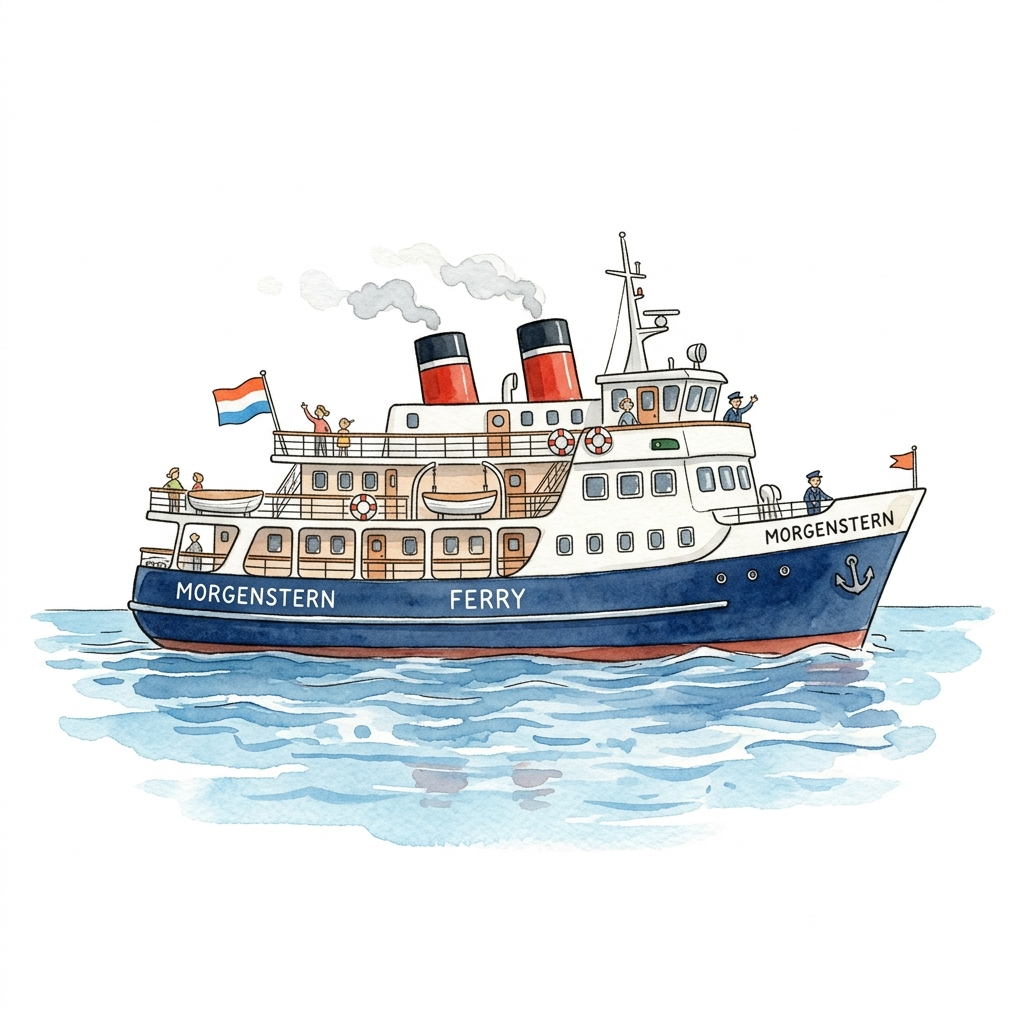
\includegraphics[width=0.85\linewidth]{vokab_300dpi/scheff.png} \\
            \vspace{0.3cm}
    }}
    \vspace{0.4em}
    \textbf{\Large D'Schëff}\\
    \small\textit{(Le bateau, le navire / The ship, boat)}
\end{minipage}
\end{noindent}

\vspace{2em}

\begin{noindent}
\begin{minipage}[t]{0.48\textwidth}
    \centering
    \textbf{\Large E Bus}
    \vspace{0.4em}
    \framebox{\parbox{0.88\linewidth}{\centering
            \vspace{0.3cm}
            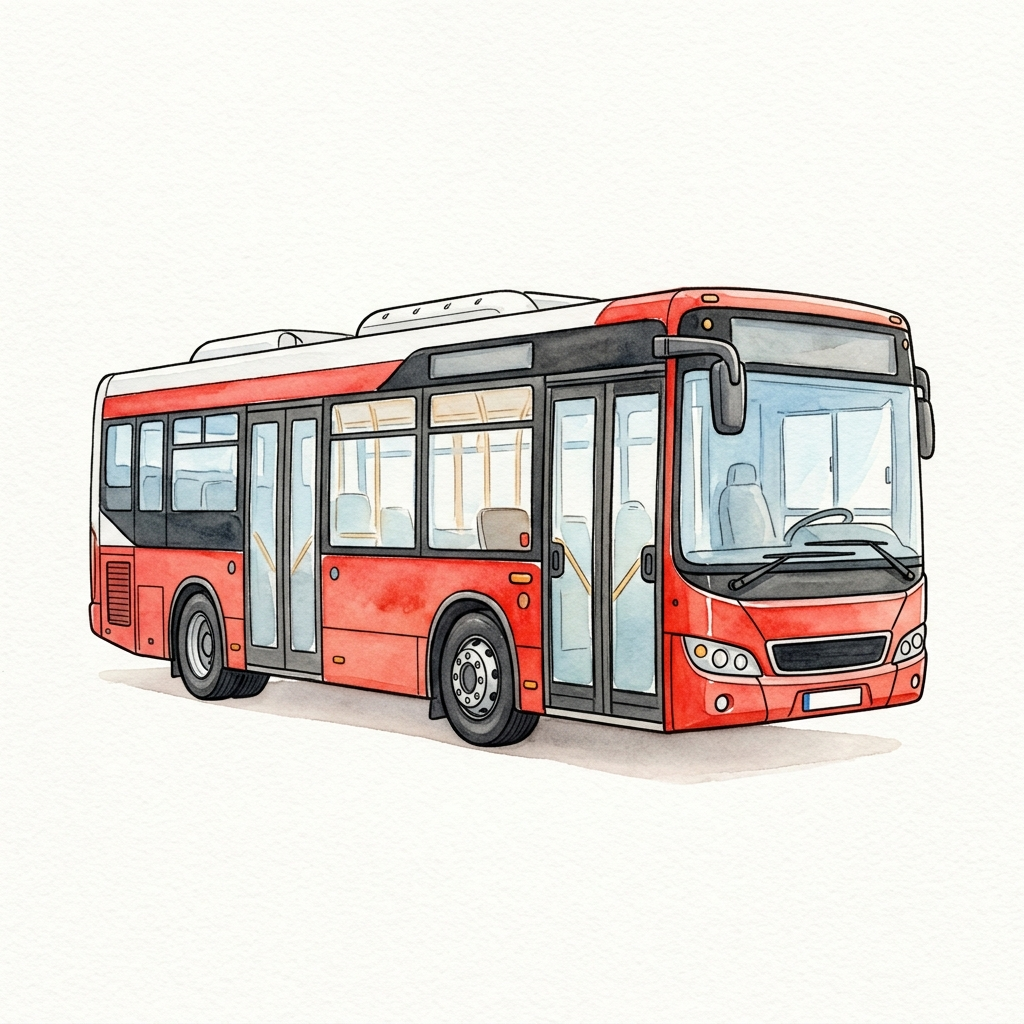
\includegraphics[width=0.85\linewidth]{vokab_300dpi/bus.png} \\
            \vspace{0.3cm}
    }}
    \vspace{0.4em}
    \textbf{\Large De Bus}\\
    \small\textit{(Le bus, l'autobus / The bus)}
\end{minipage}
\hfill
\begin{minipage}[t]{0.48\textwidth}
    \centering
    \textbf{\Large En Haus}
    \vspace{0.4em}
    \framebox{\parbox{0.88\linewidth}{\centering
            \vspace{0.3cm}
            
\includegraphics[width=0.85\linewidth]{vokab_300dpi/haus.png} \\
            \vspace{0.3cm}
    }}
    \vspace{0.4em}
    \textbf{\Large D'Haus}\\
    \small\textit{(La maison / The house)}
\end{minipage}
\end{noindent}
